\chapter{I Asked Californian Millionaires How Much Money They Lost}

This chapter is built from an interview sequence rather than a conventional classroom derivation, but it does have a real mathematical backbone. We move from headline income to drawdown, from repeated acquisition to passive cash flow, from one-person effort to organizational scale, and finally from marked wealth to usable liquidity. Since no validated board image survives for this lecture, every displayed formula below is a careful transcript-based reconstruction, kept as schematic as the interview itself.

\section{Overture: Wealth in Public, Fragility in the Background}

The episode begins with a teaser that already contains its last lesson. Before Beverly Hills, before the Lamborghini, before the G-Wagon and SoFi Stadium, we are shown the governing contrast: a year of extraordinary gain and, a few years later, a year of catastrophic loss. The host then states his method plainly. Los Angeles, he says, is one of the world's richest cities, and he is going to ask multi-millionaires not only what they made, but what they lost.

That method matters. The lecture is driven by a very small cycle of questions:
\[
\text{headline number} \;\longrightarrow\; \text{cause} \;\longrightarrow\; \text{failure} \;\longrightarrow\; \text{advice}.
\]
What gives the episode its force is that the questions are almost naive. They are so short that they force the interviewee to expose a mechanism.

The first quantitative bank is therefore an evidence bank, not yet an explanation:
\begin{equation}
Y_{\mathrm{AI}}=\$40\,\mathrm{M},\qquad
Y_{\mathrm{broker}}\approx \$8\,\mathrm{M},\qquad
Y_{\mathrm{Meltzer}}=\$34\,\mathrm{M},\qquad
L_{\mathrm{Meltzer}}>\$100\,\mathrm{M}.
\end{equation}
These are the lecture's observables. We shall not pretend they already form a model.

\begin{table}[h]
\centering
\begin{tabular}{llll}
\hline
Case & Peak figure & Stated loss or risk & Immediate mechanism \\
\hline
AI entrepreneur & \(\$40\,\mathrm{M}\) & later loss of \(95\%\) of skincare proceeds & commission-only upside \\
Homebuilder / lawyer & seven figures & risk accepted, but moderated & doubles and singles \\
Real-estate broker & \(\approx \$8\,\mathrm{M}\) & scale requires delegation & buy, rent, repeat \\
David Meltzer & \(\$34\,\mathrm{M}\) & \(>\$100\,\mathrm{M}\) lost & boom, leverage, liquidity shock \\
\hline
\end{tabular}
\caption{Transcript-backed inventory of gain, loss, and operating mechanism.}
\end{table}

The host now restarts properly in Beverly Hills. This reset is worth keeping. The episode wants the street texture to remain visible while the argument unfolds. We are not yet in general theory; we are walking up to a car and asking what made it possible.

\section{First Encounter: The Lamborghini and the Price of Variable Pay}

The first full case is an entrepreneur who says, tersely, that he is in AI, that he has been building businesses for eleven years, and that his best year brought in \(\$40\,\mathrm{M}\). The host immediately asks for financial advice, and the answer is not moderation. The answer is performance pay.

A cleaned-up version of the interview's compensation model is
\begin{equation}
C=\alpha R,\qquad \alpha \approx \frac12,
\end{equation}
where \(R\) is the revenue produced and \(C\) is the commission claimed by the producer. The doctrine is simple: suppress the salary floor and tie reward directly to output. In that spirit one has
\begin{equation}
R=0 \Longrightarrow C=0,
\qquad
R\ \text{large} \Longrightarrow C\propto R.
\end{equation}
The episode does not present this as a universal law. It presents it as one entrepreneur's way of forcing exposure and sharpening incentives.

Now the lecture makes its first essential turn. It refuses to let large earnings float free of ruin. The same speaker describes eviction, repossession, eating cheaply and secretly, a negative bank balance, and repeated failure before the later success. The rhetoric is coarse, but the structural point is exact: upside and exposure belong to the same world.

When he later says that he lost \(95\%\) of the money from a skincare sale, it is helpful to introduce a drawdown fraction
\begin{equation}
d=\frac{L}{Y},
\end{equation}
so that in this case
\begin{equation}
d_{\mathrm{skin}}=0.95,
\qquad\text{equivalently}\qquad
L_{\mathrm{skin}}=0.95\,Y_{\mathrm{skin}}.
\end{equation}
This is not a full theory of leverage or business failure. It is a clean way to register what the interview is insisting on: the relevant number is not only what one once earned, but how much of it was surrendered.

\subsection{Question \& Answer}

The host now asks the first genuine pedagogical question of the lecture: what can somebody at rock bottom actually do?

The answer comes in a sequence rather than an equation.
\begin{enumerate}
\item Read aggressively in sales, business, and self-reconstruction.
\item Recover a sense of agency; the interviewee frames this in the language of controlling reality more than people think they do.
\item Seek mentors rather than remaining closed inside one's own failed loop.
\item Change the peer environment: do not merely desire a different outcome, stand next to people already producing it.
\end{enumerate}

The social part of the answer is especially important. The speaker says that he wanted to make \(\$1000\) a day and realized none of his current circle was doing that, so he formed a mastermind group around that target. We should not over-mathematize this, but the lecture is clearly moving from interior motivation to external structure. The environment becomes part of the mechanism.

The host then recaps the interview before moving on. That recap is not disposable filler. It is how the lecture converts one case into a local theorem: a strong income claim, an extreme incentive doctrine, a collapse story, then advice for recovery.

\section{Second Encounter: Risk Without the Home Run}

The next case deliberately cools the temperature. We meet a self-made real-estate operator who has built houses, spent twenty years as a real-estate lawyer, and been in business for roughly twenty-three years. When asked for his lesson about entrepreneurship, he says: take risks. When asked to sharpen it, he gives a proverb instead of a formula: nothing ventured, nothing gained.

But then the lecture introduces a restraint that the first case lacked. The best financial advice he says he received was ``doubles and singles only.'' That is a useful phrase because it changes the optimization principle. The goal is no longer a single dramatic hit. The goal is survivable, repeatable progress.

The transcript does not supply an expected-value calculation, and we should not invent one. But it clearly prefers a regime of smaller, repeatable wins to a regime of spectacular swings that threaten continuity. The lecture is, in effect, inserting a survival filter before the next case becomes more mechanical.

The host also tries to pin down the scale of the operator's success. After some back-and-forth it settles not on eight figures, but on seven figures in a year. That hesitation is worth preserving. The chapter should not smooth every interview into a perfectly clean number. Sometimes the relevant fact is that the speaker resists the headline.

\subsection{Question \& Answer}

The host now returns to the beginner's question in a quieter register: suppose somebody is broke, coming out of school, and trying to get serious about financial freedom. What should he do first?

The answer is plain:
\begin{itemize}
\item work hard and do well in school,
\item recognize that any honest job is a real job,
\item learn from everyone with whom one does business.
\end{itemize}

This is a useful slowing-down of the lecture. After talk of Lamborghinis and eight-figure years, the episode reintroduces apprenticeship. Learning is not postponed until one arrives at a glamorous position. The lecture is telling us, in effect, that there is no shame in beginning at a small scale if one is accumulating judgment.

\section{Third Encounter: The Asset Flywheel and the Question of Scale}

The G-Wagon case is the clearest procedural model in the lecture. The interviewee says he owns a real-estate brokerage, has been in the business roughly nineteen years, has been an owner for eight, made a little over \(\$8\,\mathrm{M}\) in his best year, and became a millionaire at twenty-three. The host then asks a better question than ``How did you get rich?'' He asks how somebody today could own the same vehicle.

Now the lecture finally gives us an algorithm:
\begin{quote}
buy a property, rent it out, buy a second one, buy a house every year for four years, and by the fifth year use the passive income for the monthly payment.
\end{quote}

We may formalize that mechanism cautiously.

\begin{definition}
The asset flywheel is the transcript-derived loop in which acquired properties produce rental cash flow, rental cash flow supports further acquisition, and only after repetition is consumption funded from the stream.
\end{definition}

Let \(P_n\) be the number of acquired properties after year \(n\), and let \(F_n\) be accumulated passive cash flow. A minimal reconstruction is
\begin{align}
P_{n+1} &= P_n + 1,\\
F_{n+1} &= F_n + r_{n+1},
\end{align}
where \(r_{n+1}\) is the cash flow contributed by the newly added property.

We start from
\[
P_0=0,\qquad F_0=0.
\]
If one buys exactly one house each year for four years, then
\begin{align}
P_1&=1, & F_1&=r_1,\\
P_2&=2, & F_2&=r_1+r_2,\\
P_3&=3, & F_3&=r_1+r_2+r_3,\\
P_4&=4, & F_4&=r_1+r_2+r_3+r_4.
\end{align}
The spoken condition for the fifth year is then
\begin{equation}
F_4 \gtrsim M_{\mathrm{GW}},
\end{equation}
where \(M_{\mathrm{GW}}\) is the G-Wagon monthly payment.

A small worked example clarifies the logic without pretending to add missing data. If, purely schematically, each property contributes the same monthly cash flow \(r\), then
\[
r_1=r_2=r_3=r_4=r,
\]
and so
\begin{equation}
F_4=4r.
\end{equation}
The condition for the payment becomes
\begin{equation}
4r \gtrsim M_{\mathrm{GW}}
\qquad\Longrightarrow\qquad
r \gtrsim \frac{M_{\mathrm{GW}}}{4}.
\end{equation}
The interview does not supply rent levels, debt service, taxes, maintenance, or vacancy. So this is not a market model; it is only the clean algebra hidden inside the spoken advice.

\begin{figure}[h]
\centering
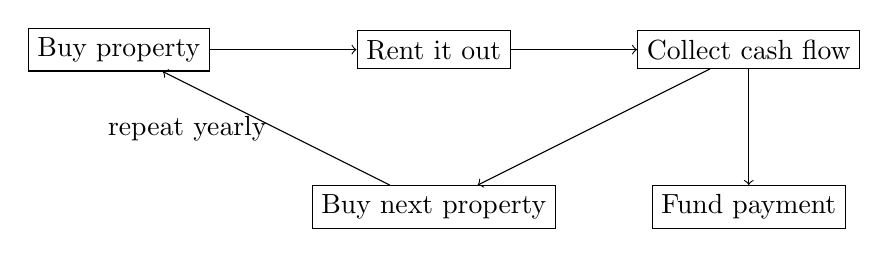
\begin{tikzpicture}[scale=1]
\node[draw, rectangle] (buy) at (0,0) {Buy property};
\node[draw, rectangle] (rent) at (4,0) {Rent it out};
\node[draw, rectangle] (flow) at (8,0) {Collect cash flow};
\node[draw, rectangle] (next) at (4,-2) {Buy next property};
\node[draw, rectangle] (pay) at (8,-2) {Fund payment};

\draw[->] (buy) -- (rent);
\draw[->] (rent) -- (flow);
\draw[->] (flow) -- (next);
\draw[->] (flow) -- (pay);
\draw[->] (next) -- node[left] {repeat yearly} (buy);
\end{tikzpicture}
\caption{Transcript-derived asset flywheel: acquisition, rent, cash flow, reinvestment, and finally funded consumption.}
\end{figure}

The host then asks the next natural question. If this becomes a serious business, what prevents it from collapsing back into one overworked person?

\subsection{Question \& Answer}

The answer is delegation. The speaker recalls seeing an entrepreneur who seemed to do almost nothing except speak with his leadership team, while every function from A to Z was managed by someone else. The lecture's scaling statement can therefore be written schematically as
\begin{equation}
\text{Scale} \Longrightarrow \text{A-to-Z functions are managed by others, not by one operator.}
\end{equation}

The logic runs in short steps.
\begin{enumerate}
\item If one person performs every function, every function shares the same bottleneck.
\item If each function is placed in other hands, the business ceases to be limited by one daily schedule.
\item The scarce skill then becomes hiring, onboarding, and retaining the right people.
\end{enumerate}

Notice how the lecture has climbed. We began with the question ``How does one afford the car?'' We are now at a different question entirely: ``How does a business stop being merely an extension of one body?''

\section{Final Encounter: Boom, Liquidity, and the Discipline of Consistency}

At SoFi Stadium the lecture reaches its most analytic case. David Meltzer says he has been in sports and entertainment for thirty-five years, that his best year was \(\$34\,\mathrm{M}\), and that this was tied to a real-estate boom. He then compresses the boom into one phrase: the real estate he had doubled in one year. We may record the statement as
\begin{equation}
V_1 \approx 2V_0,
\end{equation}
where \(V_0\) and \(V_1\) are the marked values of the same position before and after the boom. This is a shorthand, not a detailed appraisal model, but it preserves the lecture's causal sequence: appreciation first, stress later.

That stress later becomes the central mathematical event of the chapter. Meltzer explains that during the 2008 crisis he needed about \(\$5\,\mathrm{M}\), believed he had a \(\$40\,\mathrm{M}\) line of credit, and then discovered that the practically available cap was only \(\$1\,\mathrm{M}\). The point is not abstract fear of recession. The point is a mismatch:
\begin{align}
C_{\mathrm{nominal}} &= \$40\,\mathrm{M},\\
C_{\mathrm{usable}} &= \$1\,\mathrm{M},\\
N &\approx \$5\,\mathrm{M},\\
C_{\mathrm{usable}} &< N.
\end{align}

This lets us express the episode's survival logic very plainly. If \(S=1\) means ``the business can remain intact tomorrow'' and \(S=0\) means ``it cannot,'' then one schematic way to write the constraint is
\begin{equation}
S=
\begin{cases}
1, & C_{\mathrm{usable}}\ge N,\\
0, & C_{\mathrm{usable}}<N.
\end{cases}
\end{equation}
This is not a full insolvency model. It is the minimal algebraic skeleton of the story the speaker tells: when the needed liquidity exceeds the liquidity actually available, continuity itself comes into question.

That is why the lecture next introduces what it calls the golden rule of business:
\begin{definition}
The survival constraint is the requirement that one remain in business tomorrow before optimizing for any later gain.
\end{definition}

In prose, the order of priorities becomes
\[
\text{survival} \;\prec\; \text{growth} \;\prec\; \text{luxury},
\]
where the symbol is read not as a moral ranking but as a temporal one. Survival must be settled first.

The lecture then adds a retrospective lesson: the speaker should have asked for help from people who really understood financing and banking. That line matters because it blocks a common illusion. Wealth does not imply mastery of every relevant mechanism.

\subsection{Question \& Answer}

The host closes with the lecture's most nearly mathematical question: why does consistency compound?

The speaker's answer begins in spoken arithmetic. If we denote additive accumulation by \(A_n\) and the geometric sketch by \(G_n\), then
\begin{align}
A_n &= \underbrace{1+1+\cdots+1}_{n\text{ terms}} = n,\\
G_n &= 1+2+4+\cdots+2^{n-1}.
\end{align}
The lecture is not claiming that every real-world effort literally doubles. It is claiming that regular, daily action behaves differently from isolated bursts.

If we complete the arithmetic in the standard way, we obtain
\begin{align}
2G_n &= 2+4+\cdots+2^n,\\
2G_n-G_n &= (2+4+\cdots+2^n)-(1+2+4+\cdots+2^{n-1}),\\
G_n &= 2^n-1.
\end{align}
So the contrast becomes
\[
A_n=n,
\qquad
G_n=2^n-1.
\]
That is the cleanest mathematical rendering of the lecture's final intuition. ``Two minutes a day is worth two hours on a Saturday'' is not meant as a literal unit conversion. It means that repetition can aggregate, accelerate, and compound, while sporadic effort usually accumulates only linearly.

The reference to the rule of \(72\) should be handled in the same spirit. It is a verbal gesture toward compounding, not a derived result in the interview. The serious content is simply that consistency changes the growth law.

\begin{remark}
The final language about energy, physics, metaphysics, and quantum physics is rhetorical rather than technical. The chapter should preserve the speaker's intention while translating it into the safer vocabulary of repeated action, accumulation, acceleration, and compounding.
\end{remark}

\section{Summary}

This lecture unfolds by repeatedly lowering a simple hook into a complicated world. How much did you make? What happened that year? What did you lose? What would you tell somebody who is beginning with nothing?

Out of that sequence we can extract a coherent set of notes. The Lamborghini case gives us variable pay and drawdown. The next real-estate case inserts restraint: singles and doubles, not only home runs. The G-Wagon case gives us a true update rule: buy, rent, accumulate, repeat. The Meltzer case sharpens the whole chapter into its most durable lesson: wealth marked on paper is not the same thing as liquidity when the regime turns, and the first rule of business is to remain alive long enough for the next opportunity to matter.

What survives all of the episode's bravado is a sober order of operations. First secure continuity. Then build repeatable mechanisms. Then, if the stream is strong enough, let the stream pay for the symbol.